\begin{figure}[t]
\begin{center}
\begin{small}
\begin{sc}
\begin{tabular}{c@{\hskip2pt}c@{\hskip2pt}c|c@{\hskip2pt}c@{\hskip2pt}c}
Input&Ours&SimGlim&Input&Ours&SimGlim\\

\includegraphics[width=\smallerimg]{fig/ade/3/gt.jpg}&
\includegraphics[width=\smallerimg]{fig/ade/3/ours.jpg}&
\includegraphics[width=\smallerimg]{fig/ade/3/simglim.png}&

\includegraphics[width=\smallerimg]{fig/ade/2/gt.jpg}&
\includegraphics[width=\smallerimg]{fig/ade/2/ours.jpg}&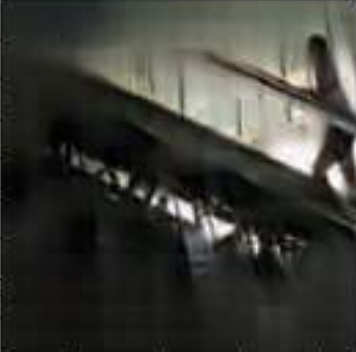
\includegraphics[width=\smallerimg]{fig/ade/2/simglim.png}\\

\includegraphics[width=\smallerimg]{fig/ade/4/gt.jpg}&
\includegraphics[width=\smallerimg]{fig/ade/4/ours.jpg}&
\includegraphics[width=\smallerimg]{fig/ade/4/simglim.png}&

\includegraphics[width=\smallerimg]{fig/ade/5/gt.jpg}&
\includegraphics[width=\smallerimg]{fig/ade/5/ours.jpg}&
\includegraphics[width=\smallerimg]{fig/ade/5/simglim.png}\\
\end{tabular}
\end{sc}
\end{small}
\end{center}
\vskip -0.1in
\caption{\textbf{Reconstruction quality for ADE20K:} Figure shows difference in reconstruction quality against SimGlim~\protect\cite{Jha2023WACV} on the ADE20K dataset. SimGlim reconstructs a single object slightly better, but our method recovers more objects in the scene.}
\label{fig:qualiative-non-retinal}
\end{figure}